\paragraph{Sơ đồ tuần tự luồng thiết lập và đồng bộ giọng nói từ ElevenLabs}

Luồng nghiệp vụ này mô tả
cách thức quản trị viên
(Admin)
kích hoạt quá trình đồng bộ các mẫu giọng nói (Voices)
từ nền tảng ElevenLabs về CSDL của dịch vụ nhân vật.

\begin{figure}[H]
\centering
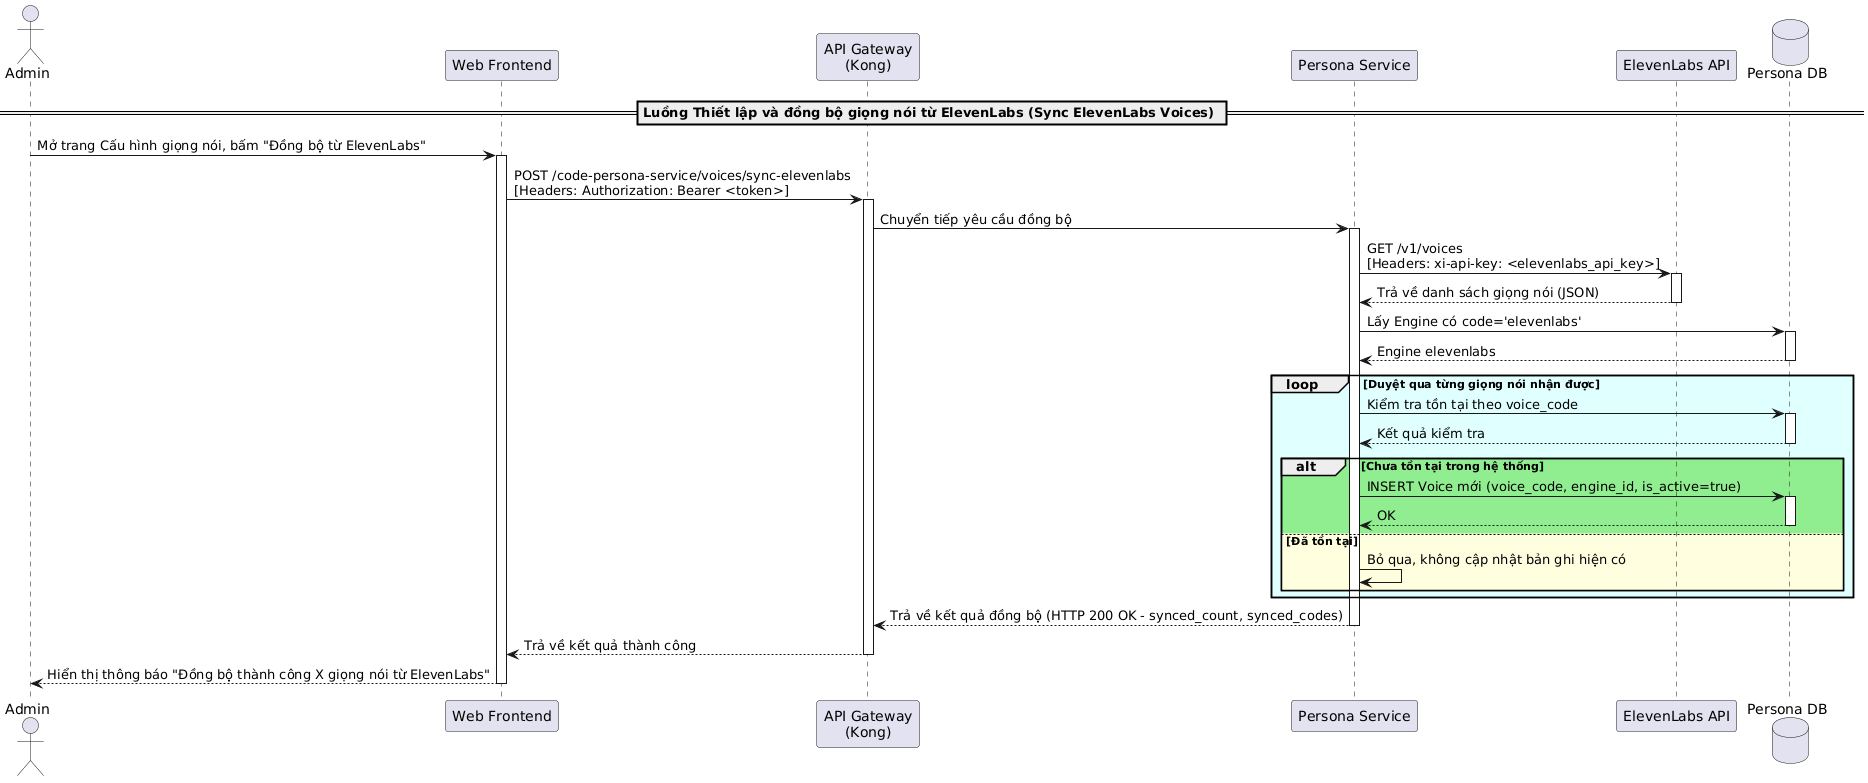
\includegraphics[width=0.95\textwidth]{contents/Sequence/UML-Sequence-AdminSyncElevenLabsVoices.png}
\caption{Sơ đồ tuần tự luồng thiết lập và đồng bộ giọng nói từ ElevenLabs}
\end{figure}

\begin{table}[H]
\centering
\renewcommand{\arraystretch}{1.3}

\begin{tabular}{|l|l|p{5cm}|}
\hline
\textbf{Thành phần} & \textbf{Phân loại} & \textbf{Vai trò trong hệ thống} \\ \hline
Admin & Actor & Quản trị viên
khởi tạo yêu cầu đồng bộ. \\ \hline
Web Frontend & Component & Giao diện web Next.js. \\ \hline
API Gateway (Kong) & Component & Cổng API chuyển tiếp các yêu cầu API. \\ \hline
Persona Service & Microservice & Tiếp nhận yêu cầu, gọi ElevenLabs API bên ngoài và thực hiện ghi dữ liệu. \\ \hline
ElevenLabs API & External Service & Cổng dịch vụ TTS bên thứ ba cung cấp danh sách giọng nói mẫu. \\ \hline
Persona Database & Database & Lưu trữ các bản ghi Voice để liên kết với các nhân vật. \\ \hline
\end{tabular}
\caption{Các thành phần tham gia luồng thiết lập và đồng bộ giọng nói từ ElevenLabs}
\end{table}

\subparagraph{Mô tả tổng quan}

\begin{itemize}

\item \textbf{Yêu cầu đồng bộ:}
Quản trị viên
chọn chức năng đồng bộ giọng nói từ giao diện.
Giao diện gửi yêu cầu đồng bộ đến dịch vụ quản lý nhân vật.

\item \textbf{Gọi dịch vụ bên ngoài:}
Dịch vụ nhân vật
gửi yêu cầu lấy danh sách giọng nói
từ nhà cung cấp dịch vụ giọng nói bên ngoài ElevenLabs bằng khóa kết nối của hệ thống.

\item \textbf{Xử lý và lưu trữ:}
Nhà cung cấp ElevenLabs phản hồi danh sách các giọng nói có sẵn.
Dịch vụ nhân vật lọc theo định danh nhà cung cấp, kiểm tra sự tồn tại của từng giọng nói
trong CSDL dựa trên định danh: nếu chưa có thì thêm mới giọng nói vào CSDL,
nếu đã có thì bỏ qua không cập nhật.

\item \textbf{Hoàn tất:}
Dịch vụ nhân vật phản hồi kết quả gồm số lượng giọng nói đã đồng bộ
và danh sách định danh giọng nói về giao diện để thông báo cho quản trị viên.

\end{itemize}
